\documentclass[a4paper,12pt]{article}
\usepackage{amsmath}
\usepackage{amssymb}
\usepackage[polish]{babel}
\usepackage{polski}
\usepackage[utf8]{inputenc}
\usepackage{indentfirst}
\usepackage{geometry}
\usepackage{array}
\usepackage[pdftex]{color,graphicx}
\usepackage{subfigure}
\usepackage{afterpage}
\usepackage{setspace}
\usepackage{color}
\usepackage{wrapfig}
\usepackage{listings}
\usepackage{datetime}
\usepackage[outdir=./]{epstopdf}

\renewcommand{\onehalfspacing}{\setstretch{1.6}}

\geometry{tmargin=2.5cm,bmargin=2.5cm,lmargin=2.5cm,rmargin=2.5cm}
\setlength{\parindent}{1cm}
\setlength{\parskip}{0mm}

\newenvironment{lista}{
\begin{itemize}
  \setlength{\itemsep}{1pt}
  \setlength{\parskip}{0pt}
  \setlength{\parsep}{0pt}
}{\end{itemize}}

\newcommand{\linia}{\rule{\linewidth}{0.4mm}}

\definecolor{lbcolor}{rgb}{0.95,0.95,0.95}
\lstset{
    backgroundcolor=\color{lbcolor},
    tabsize=4,
  language=C++,
  captionpos=b,
  tabsize=3,
  frame=lines,
  numbers=left,
  numberstyle=\tiny,
  numbersep=5pt,
  breaklines=true,
  showstringspaces=false,
  basicstyle=\footnotesize,
  identifierstyle=\color{magenta},
  keywordstyle=\color[rgb]{0,0,1},
  commentstyle=\color{Darkgreen},
  stringstyle=\color{red}
  }

\begin{document}

\noindent
\begin{tabular}{|c|p{11cm}|c|} \hline 
Grupa 1 & Kordian Kurdziel, Mateusz Maciejak & \ddmmyyyydate\today \tabularnewline
\hline 
\end{tabular}


\section*{Zadanie 1 - Rozmycie Gaussa w OpenMP}

Zadanie programu było rozmycie obrazu podanego na wejściu za pomocą algorytmu Gaussa z maską 5x5. W celu poprawy wydajności programu do zrównoleglenia jego działania należało wykorzystać OpenMP.

Poniższy fragment kodu w pierwszej pętli for jest wykonywany równolegle w oddzielnych wątkach, dzięki zastosowaniu dyrektywy pragma omp parallel for. Wartość każdego kanału RGB jest liczona oddzielnie w funkcji calculateNewPixelChannelValue()
\begin{lstlisting}
#pragma omp parallel for default(shared) private(i,j) schedule(runtime) num_threads(threadsNumber)
for (i = margin; i < inputImg.rows - margin; i++) {
	for (j = margin; j < inputImg.cols - margin; j++) {
		rgbOutputChannels[0].at<uchar>(i,j) = calculateNewPixelChannelValue(rgbInputChannels[0], i, j);
		rgbOutputChannels[1].at<uchar>(i,j) = calculateNewPixelChannelValue(rgbInputChannels[1], i, j);
		rgbOutputChannels[2].at<uchar>(i,j) = calculateNewPixelChannelValue(rgbInputChannels[2], i, j);
	}
}
\end{lstlisting}

Funkcja wylicza wartość dla każdego kanału na podstawie wagi poszczególnych pikseli maski oraz wartości tych pikseli
\begin{lstlisting}
int calculateNewPixelChannelValue(Mat channel, int row, int col) {
    int sum = 0;
    for (int i = 0; i < maskSize; ++i) {
        for (int j = 0; j < maskSize; ++j) {
            sum+= mask[i][j] * ((int) channel.at<uchar>(row + i - 2, col + j - 2));
        }
    }
    return (int) (sum / maskWeight);
}

\end{lstlisting}


Poniżej zamieszone są wykresy na dowód posiadania umiejętności obsługi pakietu biurowego Microsoft Office Excel lub LibreOffice Calc. Można tutaj również pochawlić się znajomością małego lecz potężnego programu gnuplot.

\begin{figure}[!h]
	\centering
  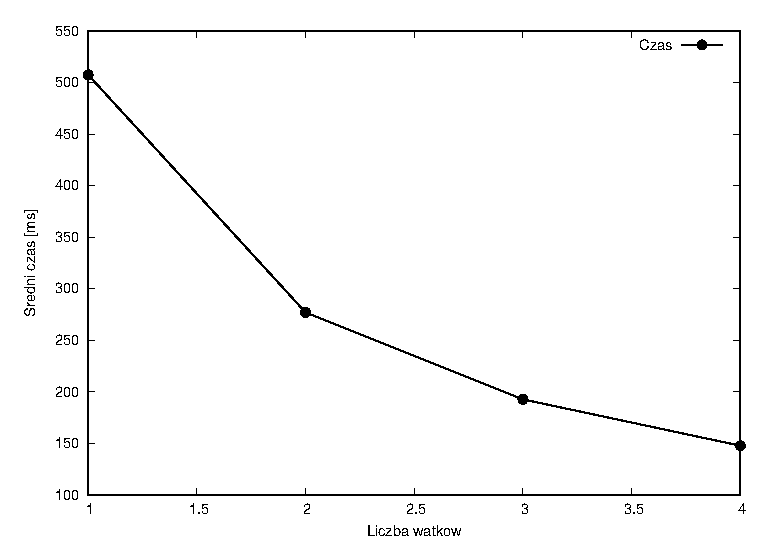
\includegraphics[width=0.6\textwidth]{dane/wykresCzas.eps}
  \caption{Wykres zależności czasu wykonywania obliczeń od liczby wątków}
\end{figure}

\begin{figure}[!h]
	\centering
  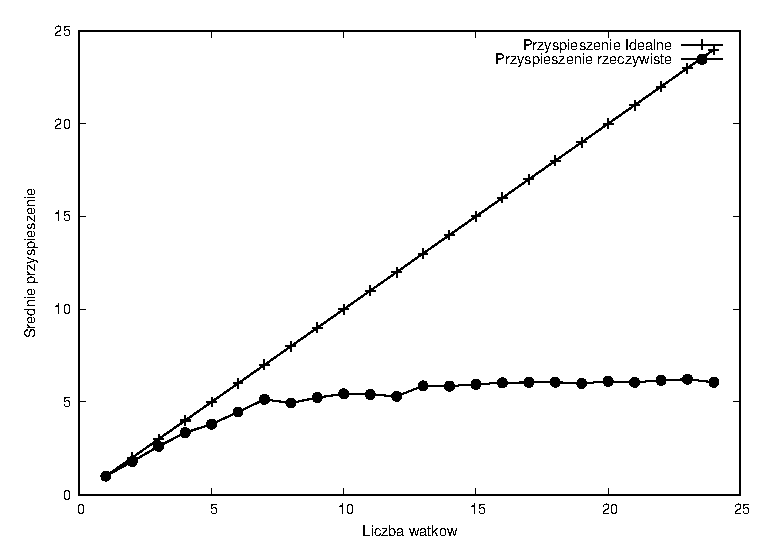
\includegraphics[width=0.6\textwidth]{dane/wykresPrzyspieszenie.eps}
  \caption{Wykres przyspieszenia działania programu w zależności od liczby wątków}
\end{figure}

W celu ułatwienia pracy Prowadzącemu warto wykresy podpisać, aby Prowadzący omyłkowo nie przyjął, że dany wykres przedstawia średnią miesięczną temperaturę w Bangladeszu na przełomie lat 1975-1982, ponieważ taki wykres byłby nieodpowiedni, przez co sprawozdanie byłoby niezaliczone. Łatwo zauważyć, że każdy wykres w przestrzeni 2D posiada dwie osie i z grzeczności należy je opisać. Osie posiadają jednostki, które też warto przytoczyć.

Czasem w sprawozdaniu warto przytoczyć kilka zalet danego rozwiązania i wypisać je jako lista:
\begin{lista}
 \item Pierwszą zaletą jest to, że jest.
 \item Druga zaleta jest również obecna.
 \item Trzecia zaleta jest już troche naciągana.
 \item Czwarta zaleta jest wadą, czyli zaletą ujemną.
\end{lista}

Jeśli zaszłaby konieczność zestawienia danych wartości w tabeli to również jest taka możliwość.

\begin{table}[!hbp]
\centering
\begin{tabular}{|p{5cm}|c|}
\hline 
Zalety & Wady \tabularnewline
\hline 
 Ładne, kolorowe & Brak\tabularnewline
 Szybkie, działające & Brak\tabularnewline
\hline
\end{tabular}
\caption{Podpis bardzo wartoścowej tabeli z danymi}
\end{table}


W sprawozdaniu muszą znaleźć się wnioski. Wnioski stanowią przesłankę, o tym iż osoba je pisząca, która ubiega się o tytuł magistra inżyniera, wie co robi. Osoba taka często jest w stanie określić czemu miało służyć dane ćwiczenie, a także ocenić w jakim stopniu udało się rozwiązać dane zagadnienie i gdzie napotkano problemy.

\end{document}
